\documentclass[10pt,mathserif]{beamer}%fleqn
\usepackage{amscd, amsthm,amssymb,latexsym}
\usepackage{xcolor}
\usepackage[utf8]{inputenc}
\usepackage[spanish]{babel}
%\usepackage{beamerthemesplit}


\usepackage{url}
\mode<presentation>{
	\usecolortheme{}
	\useinnertheme{}
	\useoutertheme{}
}

%\usepackage{enumitem}
%\setenumerate{itemsep=0.005ex,topsep=3pt}
%\setitemize{itemsep=0.005ex,topsep=3pt}

\expandafter\def\expandafter\insertshorttitle\expandafter{%
  \insertshorttitle\hfill%
  \insertframenumber\,/\,\inserttotalframenumber}


\setbeamertemplate{headline}{}
\beamertemplatenavigationsymbolsempty


%\definecolor{magenta}{RGB}{250,0,150}
%\definecolor{black}{RGB}{250,0,150}

%\definecolor{mora}{RGB}{120,0,100}
%\definecolor{pink}{RGB}{255,100,160}

%\setbeamercolor{block title example}{bg=white,fg=red}
%\setbeamercolor{structure}{bg=white,fg=red}
%\setbeamercolor{title}{bg=white,fg=red}
%\setbeamercolor{normal text}{bg=white,fg=mora}
%\setbeamercolor{frametitle}{bg=white,fg=red}

\begin{document}

%\small

\binoppenalty=10000 
\relpenalty=10000
\hyphenpenalty=5000
\exhyphenpenalty=1000


\newtheorem{observation}{Observation}
\newtheorem{conjecture}{Conjecture}
\newtheorem{belief}{Belief}
\newtheorem{question}{Question}
\newtheorem{recall}{Recordemos}




\newcommand{\Z}{{\mathbb{Z}}}
\newcommand{\N}{{\mathbb{N}}}
\newcommand{\Q}{{\mathbb{Q}}}
\newcommand{\R}{{\mathbb{R}}}
\newcommand{\floor}[1]{\lfloor #1 \rfloor } 
\newcommand{\ceil}[1]{\lceil #1 \rceil }
\newcommand{\abs}[1]{\left| #1 \right|}
\newcommand{\card}{\mbox{\raisebox{.13em}{{$\scriptstyle \#$}}}}
\newcommand{\expa}[1]{\{#1\}}
\newcommand {\base}[2]{\langle{#1};{#2}\rangle}
\newcommand{\ybar}{{\overline{y}}}
\newcommand{\xbar}{{\overline{x}}}

\newcommand{\cf}{\text{\em cf}}
\newcommand{\eps}{\varepsilon}
\newcommand{\wh}[1]{\widehat{#1}}
\newcommand{\NN}{\mathbb{N}}
\newcommand{\RR}{\mathbb{R}}
\newcommand{\uno}{\mathbbm{1}}


\newcommand{\alocc}[2]{|\!|#1|\!|_{#2}}
\newcommand{\occ}[2]{|#1|_{#2}}

\languagepath{spanish}
\deftranslation[to=spanish]{Theorem}{Teorema}
\deftranslation[to=spanish]{theorem}{teorema}
\deftranslation[to=spanish]{Definition}{Definición}
\deftranslation[to=spanish]{definition}{definición}
\deftranslation[to=spanish]{Problem}{Problema}
\deftranslation[to=spanish]{problem}{problema}
\deftranslation[to=spanish]{Corollary}{Corolario}
\deftranslation[to=spanish]{corollary}{corolario}
\deftranslation[to=spanish]{Lemma}{Lema}
\deftranslation[to=spanish]{lemma}{lema}




%\title[Del azar con dos símbolos al azar con tres símbolos]{Del azar con dos símbolos al azar con tres símbolos}
%\author[Ariel Zylber]{Ariel Zylber}
%\institute{Universidad de Buenos Aires, Argentina}
%\date{\vspace*{-3cm}\footnotesize{Tesis de Licenciatura, Universidad de Buenos Aires, Noviembre 21, 2017}}

\title{{\normalsize Tesis de Licenciatura en Ciencias de la Computación}
\\\vspace*{2cm}
\mbox{\Large Números Muy Normales}}

\author{\large Lucas Puterman
\\\vspace*{1cm}}


\date{{\footnotesize
\hspace*{-6cm}
\begin{tabular}{l}
Directora: Ver\'onica Becher \\
Departamento de Computaci\'on\\
Facultad de Ciencias Exactas y Naturales\\
 Universidad de Buenos Aires\\
20 de Noviembre, 2019
\end{tabular}
}}

\begin{frame}
\maketitle
\setcounter{framenumber}{0}
\thispagestyle{empty}
\end{frame}



\begin{frame}
\frametitle{Sobre secuencias aleatorias}

\begin{center}
  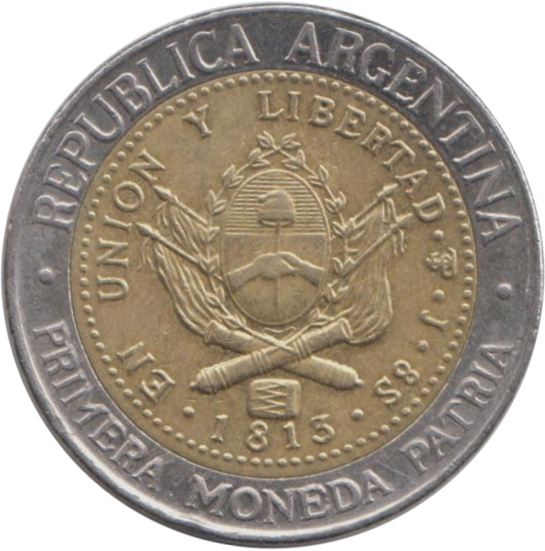
\includegraphics[scale=0.5]{imagenes/peso.jpg}
\end{center}

Supongamos que tiramos una moneda infinitas veces y anotamos un $1$ cada vez que sale cara y $0$ cada vez que sale ceca ¿Cuáles de estas secuencias es creíble que sea el resultado de este experimento?
\pause
\bigskip

\begin{itemize}
\item $11111111111111111111111111111111111\ldots$
\pause
\item $01001000100001000001000000100000001\ldots$
\pause
\item $01010101010101010101010101010101010\ldots$
\pause
\item $10000110001010001110010010110011010\ldots$
\end{itemize}
\end{frame}


\begin{frame}
\frametitle{Secuencias normales}
Podemos pensar que en una secuencia aleatoria no hay ningún patrón de~$\ell$ símbolos que sea más frecuente que otro.\\
\pause
\begin{definition}
Notamos $\occ{u}{v}$ a la \textit{cantidad de ocurrencias} de la palabra $v$ dentro de la palabra $u$.\\
\pause
\medskip
Además, notamos $u[i,j]$ a la subsecuencia de $u$ formada tomando todos los símbolos entre el $i$ y el $j$ inclusive.
\end{definition}
\pause
\medskip
Nos gustaría que para un prefijo de una secuencia aleatoria suficientemente grande, 
la cantidad de ocurrencias de cada palabra de cierta longitud sea casi la misma.
\end{frame}


\begin{frame}
\frametitle{Secuencias normales}

\begin{definition}[{{\scriptsize  Borel, 1909}}]
Dado un alfabeto $A$ y alguna secuencia infinita $u \in A^{\omega}$, 
decimos que $u$ es \textit{simplemente normal para la longitud $\ell$} 
si cada secuencia $v$ de longitud 
%$l$
\color{magenta}
$\ell$
\color{black} verifica que 
$$
\lim_{n \rightarrow \infty} \frac{\occ{u[1,\ell n]}{v}}{n} = \frac{1}{|A|^{\ell}}.
$$
\medskip
\pause

\medskip
Decimos que $u$ es \textit{normal} 
si es simplemente normal para toda longitud~$\ell \in \NN$.
 \end{definition}
\pause

\begin{problem}[{{\scriptsize  Borel, 1909}}]
Encontrar ejemplos naturales de secuencias normales. \\
Decidir si la representación en base $b$ de $\pi$, $e$ ó $\sqrt{2}$ es normal.
\end{problem}
\end{frame}


\begin{frame}
\frametitle{La secuencia de Champernowne}

  \begin{problem}
  Encontrar algún ejemplo explícito de una secuencia normal.
  \end{problem}
  \pause
  \begin{theorem}[{{\scriptsize  Champernowne, 1933}}]
  La secuencia
  $$1234567891011121314151617181920\ldots$$
  es normal 
  sobre 
  el alfabeto $A = \{0, 1, \ldots, 9\}$.
  \end{theorem}
\end{frame}

\begin{frame}
\frametitle{$champ$, La secuencia que usaremos}
  

  \begin{theorem}[{{\scriptsize  Bugeaud, 2012}}]
    Sea $A$ un alfabeto. Llamamos  $X(n)$ a la concatenación de todas las palabras de lomgitud $n$ formadas por símbolos de $A$ en orden lexicográfico.
    
    La palabra infinita $X(1)X(2)\dots$ es normal en el alfabeto $A$
  \end{theorem}

  \medskip
  \pause
  En particular, nosotros vamos a usar el alfabeto  $A=\{0,1\}$ Entonces, por ejemplo:
  $$X(2) = 00 \: 01 \: 10 \: 11$$
  \medskip
  \pause
  Entonces, los primeros símbolos de la secuencia que llamamos $champ$ son:
  $$champ = 0 \: 1 \: 00 \: 01 \: 10 \: 11 \: 000 \: 001 \: 010 \: 011 \: 100 \: 101 \: 110 \: 111 \: 0000 \: 0001 \: \dots$$


\end{frame}

\begin{frame}
\frametitle{Supernormalidad}
Sea $x$ una secuencia binaria. Sea $A^\lambda_{k,n}(x)$  la frecuencia de ocurrencia de las palabras de longitud $n$ que ocurren exactamente $k$ veces comenzando en las primeras $\floor{\lambda 2^n}$ posiciones de $x$. Es decir:
$$A^\lambda_{k,n}(x) = \frac{\#\{w: |w| = n  , |x[1...\floor{\lambda 2^n}]|_w = k\}}{2^n}$$
\pause
\begin{definition}
  Sea $\lambda$ un real mayor a cero. Decimos que la secuencia binaria $x$ es $\lambda$-supernormal si para todo entero no negativo $k$ sucede que
  $$\lim_{n\to\infty} A^\lambda_{k,n}(x) = \frac{e^{-\lambda}\lambda^k}{k!}$$

  Decimos que $x$ es supernormal si es $\lambda$-supernormal para todo $\lambda.$
\end{definition}
\end{frame}

\begin{frame}
  \frametitle{Un ejemplo para entender mejor}
  Veamos como ejemplo de juguete si la secuencia finita $x = 10011110$ es supernormal tomando $n=3$ y $\lambda = 1$.
  \pause
  Las palabras de tamaño 3 que ocurren en $x$ son:
  $$100, \; 001, \; 011,\; 111,\; 111,\; 110$$
  \pause
  Si contamos las cantidad de ocurrencias de cada palabra de tamaño 3 tenemos: 
  \begin{center}
    \begin{tabular}{|c | c|} 
    \hline
    Word & Count \\ [0.5ex] 
    \hline
    000 & 0 \\ 
    \hline
    001 & 1 \\ 
    \hline
    010 & 0 \\ 
    \hline
    011 & 1 \\ 
    \hline
    100 & 1 \\ 
    \hline
    101 & 0 \\ 
    \hline
    110 & 1 \\ 
    \hline
    111 & 2 \\ 
    \hline
   \end{tabular}
\end{center}
\end{frame}

\begin{frame}
  \frametitle{Un ejemplo para entender mejor}
  Ahora, veamos las cantidad, las frecuencias y el valor esperado para cada $k$ posible si $x$ fuera 1-supernormal.
  \pause
  \begin{center}
    \begin{tabular}{|c | c |  c| c |} 
    \hline
    $k$ & Count &  Frequency & Expected Frequency \\ [0.1ex] 
    \hline
    0 & 3 & $\frac{3}{8}$ & $e^{-1} $ \\ [0.5ex] 
    \hline
    1 & 4 &$\frac{1}{2}$ & $e^{-1} $ \\  [0.5ex] 
    \hline
    2 & 1 &$\frac{1}{8}$ & $\frac{e^{-1}}{2} $ \\  [0.5ex] 
    \hline
    3 & 0 & 0 & $\frac{e^{-1}}{3!} $ \\  [0.5ex] 
    \hline
    4 & 0 & 0 & $\frac{e^{-1}}{4!} $ \\ [0.5ex] 
    \hline
    5 & 0 & 0 & $\frac{e^{-1}}{5!} $ \\ [0.5ex] 
    \hline
    6 & 0 & 0  & $\frac{e^{-1}}{6!} $ \\ [0.5ex] 
    \hline
    7 & 0 & 0 & $\frac{e^{-1}}{7!} $ \\ [0.5ex] 
    \hline
    8 & 0 & 0 & $\frac{e^{-1}}{8!} $ \\  [0.5ex] 
    \hline
   \end{tabular}
\end{center}
\end{frame}

\begin{frame}
  \frametitle{El resultado de esta tesis}
  
  \begin{theorem}
    La noción de supernormalidad es más fuerte que la noción de normalidad.

    Es decir, los siguientes enunciados son ciertos:
    \begin{enumerate}
      \item Sea $x$ una secuencia infinita. Si $x$ es normal, no necesariamente  $x$ es supernormal. (normal $\nRightarrow$ supernormal )
      \item Sea $x$ una secuencia infinita. Si $x$ es supernormal, entonces $x$ es normal. (supernormal $\Rightarrow$ normal )
    \end{enumerate}
  \end{theorem}
\end{frame}

\begin{frame}
  \frametitle{¿Es $champ$ supernormal?}
  
  La forma más simple de ver que una secuencia normal no es supernormal es encontrar un ejemplo, y que mejor ejemplo que $champ$.

  \begin{recall}
    $X(n)$ es la concatenación de todas las palabras de longitud $n$ sobre el alfabeto $A=\{0,1\}$ en order lexicográfico.\\
    
    Llamamos $champ$ a la concatenación de  $X(n)$ para $n = 1,2,\dots$

    $$champ = 0 \: 1 \: 00 \: 01 \: 10 \: 11 \: 000 \: 001 \: 010 \: 011 \: 100 \: 101 \: 110 \: 111 \: 0000 \: 0001 \: \dots$$

  \end{recall}

  \pause
  ¿Qué sucede cuando contamos la cantidad de palabras de tamaño $n$ en los primeros $2^n$ símbolos de $champ$?
  
\end{frame}


\begin{frame}
  \frametitle{¿Es $champ$ supernormal?}
  \begin{figure}[h]
    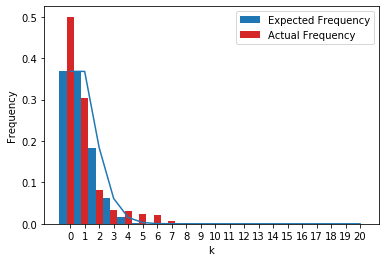
\includegraphics[width=0.75\textwidth]{imagenes/champ-16-freq.png}
    \centering
    \caption{Frecuencias observadas y esperadas en $champ$ for $n = 16$ y $\lambda = 1$.}
    \label{fig:champ-22-freq}
\end{figure}
\end{frame}

\begin{frame}
  \frametitle{¿Es $champ$ supernormal?}
  \begin{figure}[h]
    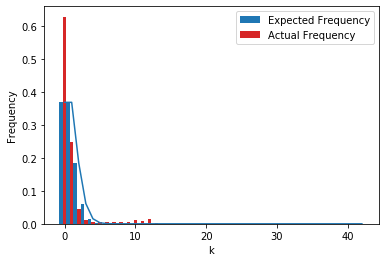
\includegraphics[width=0.75\textwidth]{imagenes/champ-22-freq.png}
    \centering
    \caption{Frecuencias observadas y esperadas en $champ$ for $n = 22$ y $\lambda = 1$.}
    \label{fig:champ-22-freq}
\end{figure}
\end{frame}

\begin{frame}
  \frametitle{Normal $\nRightarrow$ Supernormal - Idea de la demostración}
  \begin{itemize}
    \item Sabemos que $champ = X(1)X(2)X(3)\dots$
    \pause 
    \item La idea va a ser encontrar un $k$ tal que $X(k)$ sea lo suficientemente grande y este completamente contenido en $champ[1\dots 2^n]$ y analizar cuales son las palabras distintas que aparecen.
    \pause 
    \item Si tomamos $n = d + k + 1$ con $k = 2^d$, sucede que $X(k)$ está completamente contenido en $champ[1\dots 2^n]$ y además ocupa la mitad del espacio.
    \pause 
    \item Nos fijamos que pinta tienen las secuencias de longitud $d + k + 1$ que aparecen adentro de $X(k)$ y damos una cota para la cantidad de palabras distintas que pueden aparecer.
    \pause
    \item Por último resta ver que la cantidad de palabras que aparecen es mucho menor de lo necesario para que $champ$ sea supernormal.
  \end{itemize}
\end{frame}

\begin{frame}
  \frametitle{Que hay adentro de $X(k)$}
  Recordemos que definimos $k = 2^d$.
  Veamos como son las palabras de tamaño $d + k + 1$ que suceden adentro de $X(k)$. Tomemos a modo de ejemplo $k = 8$ y $d = 3$.
  \pause
  $$00000000 \qquad 00000001 \qquad 00000010 \qquad 00000011 \qquad 00000100$$
  \phantom{\parbox{\linewidth}{%
    \begin{itemize}
    \item \textcolor{red}{\underline{Caso 1:}}
    $$x = u_1 u_2 \dots u_k \quad v_1 v_2 \dots v_{d} v_{d + 1}$$
    \item \textcolor{blue}{\underline{Caso 2:}}
    $$ x = u_{k-d-1} \dots u_k \quad v_1 v_2 \dots v_k$$
    \item \textcolor{magenta}{\underline{Caso 3:}}
    $$x = u_{n+1} u_{n+2} \dots u_k \quad  v_1 v_2 \dots v_{d+n+1} $$
    con $n \in \{1,2,\dots ,k - d - 2\}$.
    \item \textcolor{orange}{\underline{Caso 4:}}
    $$ x = u_{k-d-1+n} u_{k-d+n} \dots u_k \quad v_1 v_2 \dots v_k \quad w_1 w_2 \dots w_{d+1-n}$$
    con $n \in \{1, 2, \dots , d\}$
  \end{itemize}}}\par
\end{frame} 

\begin{frame}
  \frametitle{Que hay adentro de $X(k)$}
  Recordemos que definimos $k = 2^d$.
  Veamos como son las palabras de tamaño $d + k + 1$ que suceden adentro de $X(k)$. Tomemos a modo de ejemplo $k = 8$ y $d = 3$.

  $$\textcolor{red}{(00000000 \qquad 0000)} 0001 \qquad 00000010 \qquad 00000011 \qquad 00000100$$

    \begin{itemize}
    \item \textcolor{red}{\underline{Caso 1:}}
    $$x = u_1 u_2 \dots u_k \quad v_1 v_2 \dots v_{d} v_{d + 1}$$
    \phantom{\parbox{\linewidth}{%
    \item \textcolor{blue}{\underline{Caso 2:}}
    $$ x = u_{k-d-1} \dots u_k \quad v_1 v_2 \dots v_k$$
    \item \textcolor{magenta}{\underline{Caso 3:}}
    $$x = u_{n+1} u_{n+2} \dots u_k \quad  v_1 v_2 \dots v_{d+n+1} $$
    con $n \in \{1,2,\dots ,k - d - 2\}$.
    \item \textcolor{cyan}{\underline{Caso 4:}}
    $$ x = u_{k-d-1+n} u_{k-d+n} \dots u_k \quad v_1 v_2 \dots v_k \quad w_1 w_2 \dots w_{d+1-n}$$
    con $n \in \{1, 2, \dots , d\}$
    }}\par
  \end{itemize}
\end{frame} 

\begin{frame}
  \frametitle{Que hay adentro de $X(k)$}
  Recordemos que definimos $k = 2^d$.
  Veamos como son las palabras de tamaño $d + k + 1$ que suceden adentro de $X(k)$. Tomemos a modo de ejemplo $k = 8$ y $d = 3$.

  $$0\textcolor{magenta}{(0000000 \qquad 00000)} 001 \qquad 00000010 \qquad 00000011 \qquad 00000100$$

    \begin{itemize}
    \item \textcolor{red}{\underline{Caso 1:}}
    $$x = u_1 u_2 \dots u_k \quad v_1 v_2 \dots v_{d} v_{d + 1}$$  
    \phantom{\parbox{\linewidth}{%
    \item \textcolor{blue}{\underline{Caso 2:}}
    $$ x = u_{k-d-1} \dots u_k \quad v_1 v_2 \dots v_k$$
    }}\par
    \item \textcolor{magenta}{\underline{Caso 3:}}
    $$x = u_{n+1} u_{n+2} \dots u_k \quad  v_1 v_2 \dots v_{d+n+1} $$
    con $n \in \{1,2,\dots ,k - d - 2\}$.
    \phantom{\parbox{\linewidth}{%
    \item \textcolor{cyan}{\underline{Caso 4:}}
    $$ x = u_{k-d-1+n} u_{k-d+n} \dots u_k \quad v_1 v_2 \dots v_k \quad w_1 w_2 \dots w_{d+1-n}$$
    con $n \in \{1, 2, \dots , d\}$
    }}\par
  \end{itemize}
\end{frame}

\begin{frame}
  \frametitle{Que hay adentro de $X(k)$}
  Recordemos que definimos $k = 2^d$.
  Veamos como son las palabras de tamaño $d + k + 1$ que suceden adentro de $X(k)$. Tomemos a modo de ejemplo $k = 8$ y $d = 3$.

  $$00\textcolor{magenta}{(000000 \qquad 000000)} 01 \qquad 00000010 \qquad 00000011 \qquad 00000100$$

    \begin{itemize}
    \item \textcolor{red}{\underline{Caso 1:}}
    $$x = u_1 u_2 \dots u_k \quad v_1 v_2 \dots v_{d} v_{d + 1}$$  
    \phantom{\parbox{\linewidth}{%
    \item \textcolor{blue}{\underline{Caso 2:}}
    $$ x = u_{k-d-1} \dots u_k \quad v_1 v_2 \dots v_k$$
    }}\par
    \item \textcolor{magenta}{\underline{Caso 3:}}
    $$x = u_{n+1} u_{n+2} \dots u_k \quad  v_1 v_2 \dots v_{d+n+1} $$
    con $n \in \{1,2,\dots ,k - d - 2\}$.
    \phantom{\parbox{\linewidth}{%
    \item \textcolor{cyan}{\underline{Caso 4:}}
    $$ x = u_{k-d-1+n} u_{k-d+n} \dots u_k \quad v_1 v_2 \dots v_k \quad w_1 w_2 \dots w_{d+1-n}$$
    con $n \in \{1, 2, \dots , d\}$
    }}\par
  \end{itemize}
\end{frame}

\begin{frame}
  \frametitle{Que hay adentro de $X(k)$}
  Recordemos que definimos $k = 2^d$.
  Veamos como son las palabras de tamaño $d + k + 1$ que suceden adentro de $X(k)$. Tomemos a modo de ejemplo $k = 8$ y $d = 3$.

  $$000\textcolor{magenta}{(00000 \qquad 0000000)} 1 \qquad 00000010 \qquad 00000011 \qquad 00000100$$

    \begin{itemize}
    \item \textcolor{red}{\underline{Caso 1:}}
    $$x = u_1 u_2 \dots u_k \quad v_1 v_2 \dots v_{d} v_{d + 1}$$  
    \phantom{\parbox{\linewidth}{%
    \item \textcolor{blue}{\underline{Caso 2:}}
    $$ x = u_{k-d-1} \dots u_k \quad v_1 v_2 \dots v_k$$
    }}\par
    \item \textcolor{magenta}{\underline{Caso 3:}}
    $$x = u_{n+1} u_{n+2} \dots u_k \quad  v_1 v_2 \dots v_{d+n+1} $$
    con $n \in \{1,2,\dots ,k - d - 2\}$.
    \phantom{\parbox{\linewidth}{%
    \item \textcolor{cyan}{\underline{Caso 4:}}
    $$ x = u_{k-d-1+n} u_{k-d+n} \dots u_k \quad v_1 v_2 \dots v_k \quad w_1 w_2 \dots w_{d+1-n}$$
    con $n \in \{1, 2, \dots , d\}$
    }}\par
  \end{itemize}
\end{frame}

\begin{frame}
  \frametitle{Que hay adentro de $X(k)$}
  Recordemos que definimos $k = 2^d$.
  Veamos como son las palabras de tamaño $d + k + 1$ que suceden adentro de $X(k)$. Tomemos a modo de ejemplo $k = 8$ y $d = 3$.

  $$0000\textcolor{blue}{(0000 \qquad 00000001)}  \qquad 00000010 \qquad 00000011 \qquad 00000100$$

    \begin{itemize}
    \item \textcolor{red}{\underline{Caso 1:}}
    $$x = u_1 u_2 \dots u_k \quad v_1 v_2 \dots v_{d} v_{d + 1}$$  
    \item \textcolor{blue}{\underline{Caso 2:}}
    $$ x = u_{k-d-1} \dots u_k \quad v_1 v_2 \dots v_k$$
    \item \textcolor{magenta}{\underline{Caso 3:}}
    $$x = u_{n+1} u_{n+2} \dots u_k \quad  v_1 v_2 \dots v_{d+n+1} $$
    con $n \in \{1,2,\dots ,k - d - 2\}$.
    \phantom{\parbox{\linewidth}{%
    \item \textcolor{cyan}{\underline{Caso 4:}}
    $$ x = u_{k-d-1+n} u_{k-d+n} \dots u_k \quad v_1 v_2 \dots v_k \quad w_1 w_2 \dots w_{d+1-n}$$
    con $n \in \{1, 2, \dots , d\}$
    }}\par
  \end{itemize}
\end{frame}

\begin{frame}
  \frametitle{Que hay adentro de $X(k)$}
  Recordemos que definimos $k = 2^d$.
  Veamos como son las palabras de tamaño $d + k + 1$ que suceden adentro de $X(k)$. Tomemos a modo de ejemplo $k = 8$ y $d = 3$.

  $$00000\textcolor{cyan}{(000 \qquad 00000001 \qquad 0)}  0000010 \qquad 00000011 \qquad 00000100$$

    \begin{itemize}
    \item \textcolor{red}{\underline{Caso 1:}}
    $$x = u_1 u_2 \dots u_k \quad v_1 v_2 \dots v_{d} v_{d + 1}$$  
    \item \textcolor{blue}{\underline{Caso 2:}}
    $$ x = u_{k-d-1} \dots u_k \quad v_1 v_2 \dots v_k$$
    \item \textcolor{magenta}{\underline{Caso 3:}}
    $$x = u_{n+1} u_{n+2} \dots u_k \quad  v_1 v_2 \dots v_{d+n+1} $$
    con $n \in \{1,2,\dots ,k - d - 2\}$.
    \item \textcolor{cyan}{\underline{Caso 4:}}
    $$ x = u_{k-d-1+n} u_{k-d+n} \dots u_k \quad v_1 v_2 \dots v_k \quad w_1 w_2 \dots w_{d+1-n}$$
    con $n \in \{1, 2, \dots , d\}$
  \end{itemize}
\end{frame}

\begin{frame}
  \frametitle{Que hay adentro de $X(k)$}
  Recordemos que definimos $k = 2^d$.
  Veamos como son las palabras de tamaño $d + k + 1$ que suceden adentro de $X(k)$. Tomemos a modo de ejemplo $k = 8$ y $d = 3$.

  $$000000\textcolor{cyan}{(00 \qquad 00000001 \qquad 00)}  000010 \qquad 00000011 \qquad 00000100$$

    \begin{itemize}
    \item \textcolor{red}{\underline{Caso 1:}}
    $$x = u_1 u_2 \dots u_k \quad v_1 v_2 \dots v_{d} v_{d + 1}$$  
    \item \textcolor{blue}{\underline{Caso 2:}}
    $$ x = u_{k-d-1} \dots u_k \quad v_1 v_2 \dots v_k$$
    \item \textcolor{magenta}{\underline{Caso 3:}}
    $$x = u_{n+1} u_{n+2} \dots u_k \quad  v_1 v_2 \dots v_{d+n+1} $$
    con $n \in \{1,2,\dots ,k - d - 2\}$.
    \item \textcolor{cyan}{\underline{Caso 4:}}
    $$ x = u_{k-d-1+n} u_{k-d+n} \dots u_k \quad v_1 v_2 \dots v_k \quad w_1 w_2 \dots w_{d+1-n}$$
    con $n \in \{1, 2, \dots , d\}$
  \end{itemize}
\end{frame}

\begin{frame}
  \frametitle{Que hay adentro de $X(k)$}
  Recordemos que definimos $k = 2^d$.
  Veamos como son las palabras de tamaño $d + k + 1$ que suceden adentro de $X(k)$. Tomemos a modo de ejemplo $k = 8$ y $d = 3$.

  $$0000000\textcolor{cyan}{(0 \qquad 00000001 \qquad 000)}  00010 \qquad 00000011 \qquad 00000100$$

    \begin{itemize}
    \item \textcolor{red}{\underline{Caso 1:}}
    $$x = u_1 u_2 \dots u_k \quad v_1 v_2 \dots v_{d} v_{d + 1}$$  
    \item \textcolor{blue}{\underline{Caso 2:}}
    $$ x = u_{k-d-1} \dots u_k \quad v_1 v_2 \dots v_k$$
    \item \textcolor{magenta}{\underline{Caso 3:}}
    $$x = u_{n+1} u_{n+2} \dots u_k \quad  v_1 v_2 \dots v_{d+n+1} $$
    con $n \in \{1,2,\dots ,k - d - 2\}$.
    \item \textcolor{cyan}{\underline{Caso 4:}}
    $$ x = u_{k-d-1+n} u_{k-d+n} \dots u_k \quad v_1 v_2 \dots v_k \quad w_1 w_2 \dots w_{d+1-n}$$
    con $n \in \{1, 2, \dots , d\}$
  \end{itemize}
\end{frame}

\begin{frame}
  \frametitle{Que hay adentro de $X(k)$}
  Recordemos que definimos $k = 2^d$.
  Veamos como son las palabras de tamaño $d + k + 1$ que suceden adentro de $X(k)$. Tomemos a modo de ejemplo $k = 8$ y $d = 3$.

  $$00000000 \qquad \textcolor{red}{(00000001 \qquad 0000)} 0010 \qquad 00000011 \qquad 00000100 $$

    \begin{itemize}
    \item \textcolor{red}{\underline{Caso 1:}}
    $$x = u_1 u_2 \dots u_k \quad v_1 v_2 \dots v_{d} v_{d + 1}$$
    \item \textcolor{blue}{\underline{Caso 2:}}
    $$ x = u_{k-d-1} \dots u_k \quad v_1 v_2 \dots v_k$$
    \item \textcolor{magenta}{\underline{Caso 3:}}
    $$x = u_{n+1} u_{n+2} \dots u_k \quad  v_1 v_2 \dots v_{d+n+1} $$
    con $n \in \{1,2,\dots ,k - d - 2\}$.
    \item \textcolor{cyan}{\underline{Caso 4:}}
    $$ x = u_{k-d-1+n} u_{k-d+n} \dots u_k \quad v_1 v_2 \dots v_k \quad w_1 w_2 \dots w_{d+1-n}$$
    con $n \in \{1, 2, \dots , d\}$
  \end{itemize}
\end{frame} 

\begin{frame}
  \frametitle{Que hay adentro de $X(k)$}
  Recordemos que definimos $k = 2^d$.
  Veamos como son las palabras de tamaño $d + k + 1$ que suceden adentro de $X(k)$. Tomemos a modo de ejemplo $k = 8$ y $d = 3$.

  $$11111011 \qquad 11111100 \qquad 11111101 \qquad 11111\textcolor{green}{(110 \qquad 11111111} \qquad 0\dots $$

    \begin{itemize}
    \item \textcolor{red}{\underline{Caso 1:}}
    $$x = u_1 u_2 \dots u_k \quad v_1 v_2 \dots v_{d} v_{d + 1}$$
    \item \textcolor{blue}{\underline{Caso 2:}}
    $$ x = u_{k-d-1} \dots u_k \quad v_1 v_2 \dots v_k$$
    \item \textcolor{magenta}{\underline{Caso 3:}}
    $$x = u_{n+1} u_{n+2} \dots u_k \quad  v_1 v_2 \dots v_{d+n+1} $$
    con $n \in \{1,2,\dots ,k - d - 2\}$.
    \item \textcolor{cyan}{\underline{Caso 4:}}
    $$ x = u_{k-d-1+n} u_{k-d+n} \dots u_k \quad v_1 v_2 \dots v_k \quad w_1 w_2 \dots w_{d+1-n}$$
    con $n \in \{1, 2, \dots , d\}$
    \item \textcolor{green}{\underline{Caso 5:}}
    Si $x$ comienza al final de $X(k)$ o cerca, se pueden llegar a necesitar palabras fuera de $X(k)$ para completar $d+k+1$.
  \end{itemize}
\end{frame} 

\begin{frame}
  \frametitle{La función $next(w)$}

  Definimos la siguiente función que nos va a ser útil.

  \begin{definition}
    La función $next(w) : A^n \rightarrow A^n$ se define de la siguiente manera. Si $w$ es la palabra de $n$  1s, $next(w)$ es la palabra de $n$ 0s. Si no, $next(w)$ es la palabra siguiente en orden lexicográfico.
  \end{definition}
  
  Por ejemplo,
  $$next(0000) = 0001$$
  $$next(0001) = 0010$$
  $$\vdots$$
  $$next(1110) = 1111$$
  $$next(1111) = 0000$$

\end{frame} 

\begin{frame}
  \frametitle{Análisis por caso - Caso 1}
    $$x = u_1 u_2 \dots u_k \quad v_1 v_2 \dots v_{d} v_{d + 1}$$

  Este caso representa a la ocurrencia alineada de $u$ de tamaño $k$ seguido por los primeros $d+1$ símbolos de $v$

  \begin{columns}
    \begin{column}{0.5\textwidth}
      $$( 00000000 \qquad 0000 ) \; 0001$$
      $$( 00000001 \qquad 0000 ) \; 0010$$
      $$( 00000010 \qquad 0000 ) \; 0011$$
      $$\vdots$$
      $$( 00001110 \qquad 0000 ) \; 1111$$
      $$( 00001111 \qquad 0001 ) \; 0000$$
      $$( 00010000 \qquad 0001 ) \; 0001$$
      $$\vdots$$
      $$( 11111110 \qquad 1111 ) \; 1111$$
    \end{column}
    \begin{column}{0.5\textwidth}  %%<--- here
        \begin{center}
        %  \includegraphics[width=0.5\textwidth]{image1.jpg}
         \end{center}
    \end{column}
    \end{columns}



\end{frame} 

\begin{frame}
  \frametitle{Análisis por caso - Caso 1}
    $$x = u_1 u_2 \dots u_k \quad v_1 v_2 \dots v_{d} v_{d + 1}$$

  Este caso representa a la ocurrencia alineada de $u$ de tamaño $k$ seguido por los primeros $d+1$ símbolos de $v$
  
  \begin{columns}
    \begin{column}{0.5\textwidth}
      $$( \textcolor{red}{0000}0000 \qquad \textcolor{red}{0000} ) \; 0001$$
      $$( \textcolor{red}{0000}0001 \qquad \textcolor{red}{0000} ) \; 0010$$
      $$( \textcolor{red}{0000}0010 \qquad \textcolor{red}{0000} ) \; 0011$$
      $$\vdots$$
      $$( \textcolor{red}{0000}1110 \qquad \textcolor{red}{0000} ) \; 1111$$
      $$( \textcolor{blue}{0000}\textcolor{magenta}{1111} \qquad \textcolor{cyan}{0001} ) \; 0000$$
      $$( 00010000 \qquad 0001 ) \; 0001$$
      $$\vdots$$
      $$( 11111110 \qquad 1111 ) \; 1111$$
    \end{column}
    \begin{column}{0.5\textwidth}  %%<--- here
          \pause
          $$\underbrace{\quad \textcolor{red}{A} \quad }_{d +1} \qquad \underbrace{\quad B \quad }_{k - d - 1}  \qquad \textcolor{red}{A}$$
          $$\underbrace{\quad \textcolor{blue}{A} \quad }_{d +1} \qquad \underbrace{ \textcolor{magenta}{11 \dots 1  }}_{k - d - 1}  \qquad \textcolor{cyan}{next(A)} $$
          \pause
          Del primer esquema tenemos:
          $$2^{d + 1}  (2^{k - d - 1} - 1) =  2^k - \frac{1}{2\cdot2^{d} }$$
        
          Mientras que del segundo:
          $$2^{d + 1}   - 1$$

          Juntos son menos que $2^k -  2\cdot 2^d$
    \end{column}
    \end{columns}
\end{frame} 

\begin{frame}
  \frametitle{Análisis por caso - Caso 2}
  $$ x = u_{k-d-1} \dots u_k \quad v_1 v_2 \dots v_k$$

  Este caso representa a la ocurrencia alineada de $v$ de tamaño $k$ precedida por los últimos $d+1$ símbolos de $u$
  
  \begin{columns}
    \begin{column}{0.5\textwidth}
      $$0000 \; (0000 \qquad 00000001)$$
      $$0000 \; (\; 0001 \qquad 00000010)$$
      $$\vdots$$
      $$0000 \; (1111 \qquad 10000000)$$
      $$1000 \; (0000 \qquad 10000001)$$
      $$\vdots$$
      $$1111 \; (1110 \qquad 11111111)$$
    \end{column}
    \begin{column}{0.5\textwidth}  %%<--- here
          
    \end{column}
    \end{columns}
\end{frame} 

\begin{frame}
  \frametitle{Análisis por caso - Caso 2}
  $$ x = u_{k-d-1} \dots u_k \quad v_1 v_2 \dots v_k$$

  Este caso representa a la ocurrencia alineada de $v$ de tamaño $k$ precedida por los últimos $d+1$ símbolos de $u$
  
  \begin{columns}
    \begin{column}{0.5\textwidth}
      $$0000 \; (\textcolor{red}{0000} \qquad 0000\textcolor{blue}{0001})$$
      $$0000 \; (\; \textcolor{red}{0001} \qquad 0000\textcolor{blue}{0010})$$
      $$\vdots$$
      $$0000 \; (\textcolor{red}{1111} \qquad 1000\textcolor{blue}{0000})$$
      $$1000 \; (\textcolor{red}{0000} \qquad 1000\textcolor{blue}{0001})$$
      $$\vdots$$
      $$1111 \; (\textcolor{red}{1110} \qquad 1111\textcolor{blue}{1111})$$
    \end{column}
    \begin{column}{0.5\textwidth}  %%<--- here
          \pause
          $$\underbrace{\quad \textcolor{red}{A} \quad }_{d +1} \qquad \underbrace{\quad B \quad }_{k - d - 1}  \qquad \textcolor{blue}{next(A)}$$
          \pause
          Este esquema nos da:
          $$(2^{d + 1} 2^{k-d})-1=  2 \cdot 2^k - 1$$
          palabras distintas.

          Que es menos que  $2 \cdot 2^k$ palabras distintas.
    \end{column}
    \end{columns}
\end{frame} 

\begin{frame}
  \frametitle{Análisis por caso - Caso 3}
  $$x = u_{n+1} u_{n+2} \dots u_k \quad  v_1 v_2 \dots v_{d+n+1}   \qquad n \in \{1,2,\dots ,k - d - 2\}  $$
  Este caso representa cuando los $k + d + 1$ símbolos son tomados de dos palabras $u$ y $v$ de longitud $k$ y ninguna de las dos está completas.
  Ejemplo tomando $n = 3$, $k = 8$ y $d = 3$.
  \begin{columns}
    \begin{column}{0.5\textwidth}
        $$000\; (0000\; 0 \qquad 000 \;0000 ) \;1$$
        $$000\; (0000\; 1 \qquad 000 \;0001 ) \;0$$
        $$000\; (0001\; 0 \qquad 000 \;0001 ) \;1$$
        $$000\; (0001\; 1 \qquad 000 \;0010 ) \;0$$
        $$\vdots$$
        $$111\; (1110\; 1 \qquad 111 \;1111 ) \;0$$
        $$111\; (1111\; 0 \qquad 111 \;1111 ) \;1$$
    \end{column}
    \begin{column}{0.5\textwidth}  %%<--- here

    \end{column}
    \end{columns}
\end{frame}

\begin{frame}
  \frametitle{Análisis por caso - Caso 3}
  $$x = u_{n+1} u_{n+2} \dots u_k \quad  v_1 v_2 \dots v_{d+n+1}   \qquad n \in \{1,2,\dots ,k - d - 2\}  $$
  Este caso representa cuando los $k + d + 1$ símbolos son tomados de dos palabras $u$ y $v$ de longitud $k$ y ninguna de las dos está completas.
  Ejemplo tomando \textbf{$n = 1$}, $k = 8$ y $d = 3$.
  \begin{columns}
    \begin{column}{0.5\textwidth}
      \begin{small}

      $$0\; (0000\; 000 \qquad 0 \;0000 ) \;001$$
      $$0\; (0000 \;001 \qquad 0 \;0000 ) \;010$$
      $$\vdots$$
      $$0\; (0001 \;110 \qquad 0 \;0001 ) \;111$$
      $$0\; (0001 \;111 \qquad 0 \;0010 ) \;000$$
      $$0\; (0010 \;000 \qquad 0 \;0010 ) \;001$$
      $$\vdots$$
      $$1\; (1111 \;101 \qquad 1 \;1111 ) \;110$$
      $$0\; (1111 \;110 \qquad 1 \;1111 ) \;111$$
      \end{small}
    \end{column}
    \begin{column}{0.5\textwidth}  %%<--- here
          
    \end{column}
    \end{columns}
\end{frame}

\begin{frame}
  \frametitle{Análisis por caso - Caso 3}
  $$x = u_{n+1} u_{n+2} \dots u_k \quad  v_1 v_2 \dots v_{d+n+1}   \qquad n \in \{1,2,\dots ,k - d - 2\}  $$
  Este caso representa cuando los $k + d + 1$ símbolos son tomados de dos palabras $u$ y $v$ de longitud $k$ y ninguna de las dos está completas.
  Ejemplo tomando $n = 1$, $k = 8$ y $d = 3$.
  \begin{columns}
    \begin{column}{0.5\textwidth}
      \begin{small}

      $$0\; (\textcolor{red}{0000}\; 000 \qquad 0 \;\textcolor{red}{0000} ) \;001$$
      $$0\; (\textcolor{red}{0000} \;001 \qquad 0 \;\textcolor{red}{0000} ) \;010$$
      $$\vdots$$
      $$0\; (\textcolor{red}{0001} \;110 \qquad 0 \;\textcolor{red}{0001} ) \;111$$
      $$0\; (\textcolor{red}{0001} \;\textcolor{blue}{111} \qquad 0 \;\textcolor{cyan}{0010} ) \;000$$
      $$0\; (\textcolor{red}{0010} \;000 \qquad 0 \;\textcolor{red}{0010} ) \;001$$
      $$\vdots$$
      $$1\; (\textcolor{red}{1111} \;101 \qquad 1 \;\textcolor{red}{1111} ) \;110$$
      $$0\; (\textcolor{red}{1111} \;110 \qquad 1 \;\textcolor{red}{1111} ) \;111$$
      \end{small}
    \end{column}
    \begin{column}{0.5\textwidth}  %%<--- here
      \pause
      $$\underbrace{\quad \textcolor{red}{A} \quad }_{d +1} \qquad \underbrace{\quad B \quad }_{k - d - 1}  \qquad \textcolor{red}{A}$$
      $$\underbrace{\quad \textcolor{red}{A} \quad }_{d +1} \qquad \underbrace{\; \textcolor{blue}{11\dots1}C \; }_{k - d - 1}  \qquad \textcolor{cyan}{next(A)}$$

      Pero el primer esquema ya lo contamos en el caso 1 y el segundo esquema es un caso particular de uno de los esquemas del caso 2.
      
      Por lo que el caso 3 no nos arroja nuevas palabras.
    \end{column}
    \end{columns}
\end{frame}

\begin{frame}
  \frametitle{Análisis por caso - Caso 4}
  $$ x = u_{k-d-1+n} u_{k-d+n} \dots u_k \quad v_1 v_2 \dots v_k \quad w_1 w_2 \dots w_{d+1-n} $$
  con $n \in \{1, 2, \dots , d\}$

  Este caso representa cuando los $k + d + 1$ símbolos son tomados de tres palabras consecutivas $u$, $v$ y $w$ de longitud $k$ de los cuales $k$ símbolos son tomados de $v$ y los restantes de $u$ y $w$.
  Ejemplo tomando $n = 1$, $k = 8$ y $d = 3$.
  \begin{columns}
    \begin{column}{0.5\textwidth}
      \begin{small}

        $$0000000\; (0 \qquad 000 \; 0000 \; 1 \qquad 000) \: 00010$$
        $$0000000\; (1 \qquad 000 \; 0001 \; 0 \qquad 000) \: 00011$$
        $$\vdots$$
        $$0011111\; (0 \qquad 001 \; 1111 \; 1 \qquad 001) \: 10000$$
        $$0011111\; (1 \qquad 010 \; 0000 \; 0 \qquad 010) \: 00001$$
        $$\vdots$$
        $$1111110\; (1 \qquad 111 \; 1111 \; 0 \qquad 111) \: 11111$$
      \end{small}
    \end{column}
    \begin{column}{0.5\textwidth}  %%<--- here
    \end{column}
    \end{columns}
\end{frame}

\begin{frame}
  \frametitle{Análisis por caso - Caso 4}
  $$ x = u_{k-d-1+n} u_{k-d+n} \dots u_k \quad v_1 v_2 \dots v_k \quad w_1 w_2 \dots w_{d+1-n} $$
  con $n \in \{1, 2, \dots , d\}$

  Este caso representa cuando los $k + d + 1$ símbolos son tomados de tres palabras consecutivas $u$, $v$ y $w$ de longitud $k$ de los cuales $k$ símbolos son tomados de $v$ y los restantes de $u$ y $w$.
  Ejemplo tomando $\textbf{n = 2}$, $k = 8$ y $d = 3$.
  \begin{columns}
    \begin{column}{0.5\textwidth}
      \begin{small}

        $$000000\; (00 \qquad 00 \; 0000 \; 01 \qquad 00) \: 000010$$
$$000000\; (01 \qquad 00 \; 0000 \; 10 \qquad 00) \: 000011$$
$$\vdots$$
$$001111\; (01 \qquad 00 \; 1111 \; 10 \qquad 00) \: 111111$$
$$001111\; (10 \qquad 00 \; 1111 \; 11 \qquad 01) \: 000000$$
$$001111\; (11 \qquad 01 \; 0000 \; 00 \qquad 01) \: 000001$$
$$\vdots$$
$$111111\; (01 \qquad 11 \; 1111 \; 10 \qquad 11) \: 111111$$
      \end{small}
    \end{column}
    \begin{column}{0.5\textwidth}  %%<--- here
    \end{column}
    \end{columns}
\end{frame}

\begin{frame}
  \frametitle{Análisis por caso - Caso 4}
  $$ x = u_{k-d-1+n} u_{k-d+n} \dots u_k \quad v_1 v_2 \dots v_k \quad w_1 w_2 \dots w_{d+1-n} $$
  con $n \in \{1, 2, \dots , d\}$
  \begin{columns}
    \begin{column}{0.5\textwidth}

        $$000000\; (\textcolor{red}{00} \quad \textcolor{blue}{00} \; 0000 \; \textcolor{red}{01} \quad \textcolor{blue}{00}) \: 000010$$
        $$000000\; (\textcolor{red}{01} \quad \textcolor{blue}{00} \; 0000 \; \textcolor{red}{10} \quad \textcolor{blue}{00}) \: 000011$$
        $$\vdots$$
        $$001111\; (\textcolor{red}{01} \quad \textcolor{blue}{00} \; 1111 \; \textcolor{red}{10} \quad \textcolor{blue}{00}) \: 111111$$
        $$001111\; (\textcolor{cyan}{10} \quad \textcolor{blue}{00} \; \textcolor{magenta}{1111} \; \textcolor{red}{11} \quad \textcolor{gray}{01}) \: 000000$$
        $$001111\; (\textcolor{red}{11} \quad \textcolor{blue}{01} \; 0000 \; \textcolor{red}{00} \quad \textcolor{blue}{01}) \: 000001$$
        $$\vdots$$
        $$111111\; (\textcolor{red}{01} \quad \textcolor{blue}{11} \; 1111 \; \textcolor{red}{10} \quad \textcolor{blue}{11}) \: 111111$$
    \end{column}
    \begin{column}{0.5\textwidth}  %%<--- here
      \pause
      \begin{footnotesize}
        $$\underbrace{\quad \textcolor{red}{A} \quad }_{n} \quad \underbrace{\quad \textcolor{blue}{B} \quad }_{d + 1 - n}  \quad \underbrace{\quad C \quad }_{k-d+1} \quad \textcolor{red}{next(A)} \quad \textcolor{blue}{B}$$

        $$\underbrace{\quad \textcolor{cyan}{1\dots10} \quad }_{n} \; \underbrace{\quad \textcolor{blue}{B} \quad }_{d + 1 - n}  \; \underbrace{\; \textcolor{magenta}{1\dots1} \; }_{k-d+1} \quad \textcolor{red}{n(A)} \quad \textcolor{gray}{n(B)}$$
        
        Para el primer esquema tenemos $2^k \sum_{n=1}^{d} \frac{2^n - 1}{2^n}$

        Para el segundo esquema $ 2 \cdot 2^d \sum_{n=1}^{d} 2^{- n}$

        Juntos son menos que 
        $$d2^k + 2 \cdot 2^d$$
      \end{footnotesize}
    \end{column}
    \end{columns}
\end{frame}


\begin{frame}
  \frametitle{Acotando palabras distintas en $champ$}
  Si $champ$ fuera supernormal, la frecuencia experada de palabras que aparecen una o más veces en los primeros $2^n$ símbolos debería satisfacer:
$$\lim_{n\to\infty} \frac{\#\{w: |w| = n  , |champ[1...2^n]|_w > 0\}}{2^n}  = 1 - e^{-1}$$
\pause
Sabemos que $X(k)$ ocupa la mitad de las palabras de los primeros $2^{d+k+1}$ símbolos de $champ$.
Si analizamos lo que sucede en las palabras de longitud $d+k+1$ usando las cotas que calculamos en los diferentes casos, y asumimos que la mitad restante ($2^{d+k} + d + k - 1$) son todas diferentes, entonces:
  $$&\lim_{d\to\infty} \frac{\#\{w : |w| = d+k+1, |champ[1 \dots 2^{d+k+1}]|_w > 0 \}}{2^{d+k+1}} <$$
  $$&\lim_{d\to\infty} \frac{ \textrm{Case 1} + \textrm{Case 2}+ \textrm{Case 4} + \textrm{Case 5} + \textrm{other half}}{2^{d+k+1}} =$$

  \pause 

    $$&\lim_{d\to\infty} \frac{(2^k - 2\cdot 2^d) + (2 \cdot 2^k)+ (d2^k + 2 \cdot 2^d) + (2d+k+1) + (2^{d+k}) }{2^{d+k+1}} =$$
    $$\lim_{d\to\infty} \frac{3}{2k} + \frac{d}{2k} + \frac{d}{k2^{k}} + \frac{1}{2\cdot2^{k}} + \frac{1}{2k2^{k}} + \frac{1}{2} = \frac{1}{2}$$
    $$< 1 - e^{-1}$$

\end{frame}

\begin{frame}
  \frametitle{Acotando palabras distintas en $champ$}
  Finalmente, si en $champ$ consideramos que los $n$'s tales que $n = d + 2^d + 1$ son una subsecuencia de $n=1,2,\dots$, podemos afirmar que si:
  $$\lim_{n\to\infty} \frac{\#\{w: |w| = n  , |champ[1...2^n]|_w > 0\}}{2^n}$$
  existe, este no es $1 - e^{-1}$.

\begin{corollary}
Si $x$ es normal, no necesariamente $x$ es supernormal.
\end{corollary}
\end{frame}



\end{document}


